\documentclass[DIN, pagenumber=false, fontsize=11pt, parskip=half]{scrartcl}

\usepackage{amsmath}
\usepackage{amsfonts}
\usepackage{amssymb}
\usepackage{enumitem}
\usepackage[utf8]{inputenc} 
\usepackage[ngerman]{babel} 
\usepackage[T1]{fontenc} 
\usepackage{pgfplots}
\usepackage{xcolor}
\usepackage{listings}
\usepackage{float}
\usepackage{graphicx}
\usepackage{svg}

\definecolor{mygreen}{RGB}{28,172,0} % color values Red, Green, Blue
\definecolor{mylilas}{RGB}{170,55,241}

\lstset{language=Matlab,%
    %basicstyle=\color{red},
    breaklines=true,%
    morekeywords={matlab2tikz},
    keywordstyle=\color{blue},%
    morekeywords=[2]{1}, keywordstyle=[2]{\color{black}},
    identifierstyle=\color{black},%
    stringstyle=\color{mylilas},
    commentstyle=\color{mygreen},%
    showstringspaces=false,%without this there will be a symbol in the places where there is a space
    numbers=left,%
    numberstyle={\tiny \color{black}},% size of the numbers
    numbersep=9pt, % this defines how far the numbers are from the text
    emph=[1]{for,end,break},emphstyle=[1]\color{red}, %some words to emphasise
    %emph=[2]{word1,word2}, emphstyle=[2]{style},    
}

\title{Computer Vision I}
\author{Tim Luchterhand, Paul Nykiel (Group 17)}

\begin{document}
    \maketitle
    \section{Filter Algebra}
    \subsection{}
    Without loss of generality choose an image $I \in [0,255]$ with size $3 \times 3$. 
    
    The maximum value for $I_{22}$ is achieved by weighting all positive values in the filter with $255$ and all negativ values with $0$. This results in image \eqref{eq:imgMax}. With this image the maximum output value is $2 \cdot 255 + 2 \cdot 255 + 1 \cdot 255 = 1275$.
    \begin{equation}
        \label{eq:imgMax}
        I_{max} = \begin{pmatrix}
            0 & 0 & 0 \\
            0 & 0 & 255 \\
            0 & 255 & 255
        \end{pmatrix}
    \end{equation}
    
    The minimum value for $I_{22}$ is achieved by weighting all positive values in the filter with $0$ and all negativ values with $255$. This results in image \eqref{eq:imgMin}. With this image the maximum output value is $-2 \cdot 255 + (-2) \cdot 255 + (-1) \cdot 255 = -1275$.
    \begin{equation}
        \label{eq:imgMin}
        I_{max} = \begin{pmatrix}
            255 & 255 & 0 \\
            255 & 0 & 0 \\
            0 & 0 & 0
        \end{pmatrix}
    \end{equation}

    \subsection{}
    \begin{eqnarray*}
        I &=& (1\ 2) \\
        H &=& (1\ -1) \\
        \alpha = 255
    \end{eqnarray*}
    With these values calculate the convolution (the values are continued with $0$):
    \begin{eqnarray*}
        (\alpha \cdot I) * H &=& 
        (255\ 255) * (1\ -1) =
        (255\ 0\ 0) \\
        \alpha \cdot (I * H) &=&
        255 \cdot (1\ 1\ 0) =
        (255\ 255\ 0) \\
        &\Rightarrow& (\alpha \cdot I) * H  \alpha \cdot (I * H)
    \end{eqnarray*}
    As shown by the contradiction above the linearity does not hold for clamped values.

    \subsection{}
    Matlab Code:
    \lstinputlisting[lastline=20]{sh02ex01.m}              
    \begin{figure}[H]
        \centering
        \includegraphics[trim = {0 13cm 27cm 0}, clip,width=\textwidth]{lenaEdge1.eps}
        \caption{Output of the Matlab script}
    \end{figure}
    The filter highlights strong edges in the diagonal axis (north-west to south-east) by calculating
    an approximitation of the derivative in this direction.

    \subsection{}
    \lstinputlisting[firstline=22, firstnumber=22]{sh02ex01.m}              
    \begin{figure}[H]
        \centering
        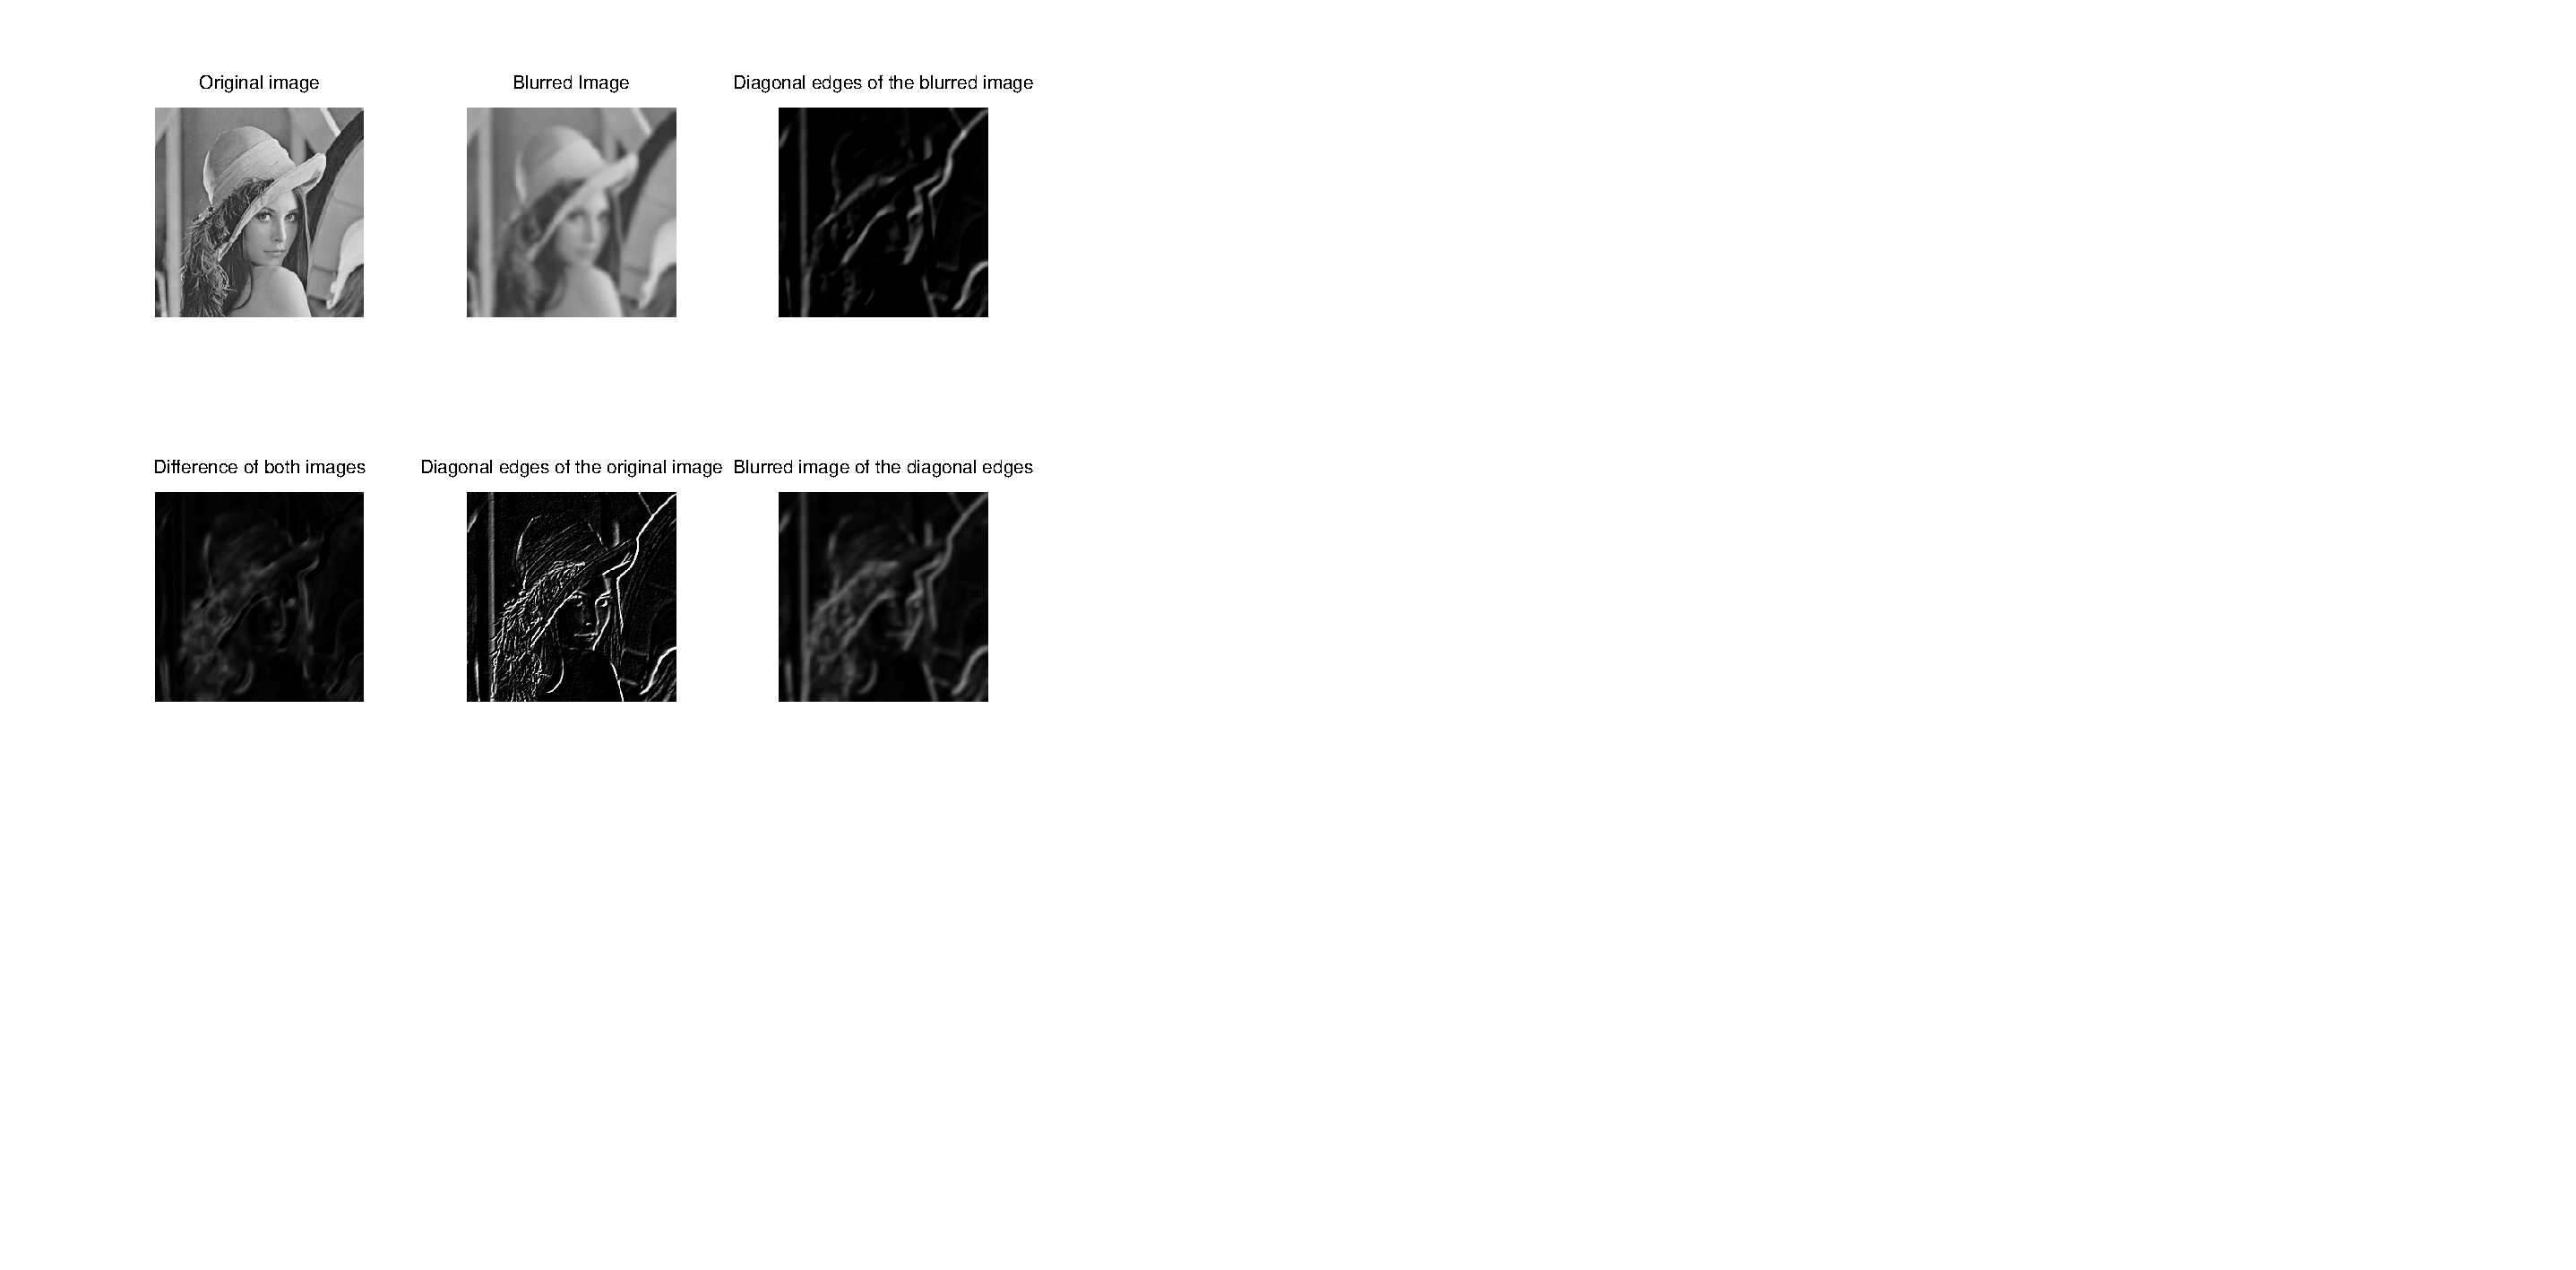
\includegraphics[trim = {0 10cm 27cm 0}, clip,width=\textwidth]{lenaEdge2.eps}
        \caption{Output of the second part of the Matlab script}
    \end{figure}

    The second image looks slighly more detailed. When using clamped images the convolution producrt is no longer commutative.


    \section{Discrete Fourier Transform}
    \subsection{}
    \lstinputlisting[lastline=16]{sh02ex02.m}              
    \subsection{}
    The $u$th coefficient (starting at zero) corresponds to a frequency of
    \begin{equation*}
        f(u) = 2 \cdot \pi \cdot \frac{u}{N} = \frac{\pi \cdot u}{2}
    \end{equation*}
    \lstinputlisting[firstline=17,firstnumber=17,lastline=26]{sh02ex02.m}              
    \begin{figure}[H]
        \centering
        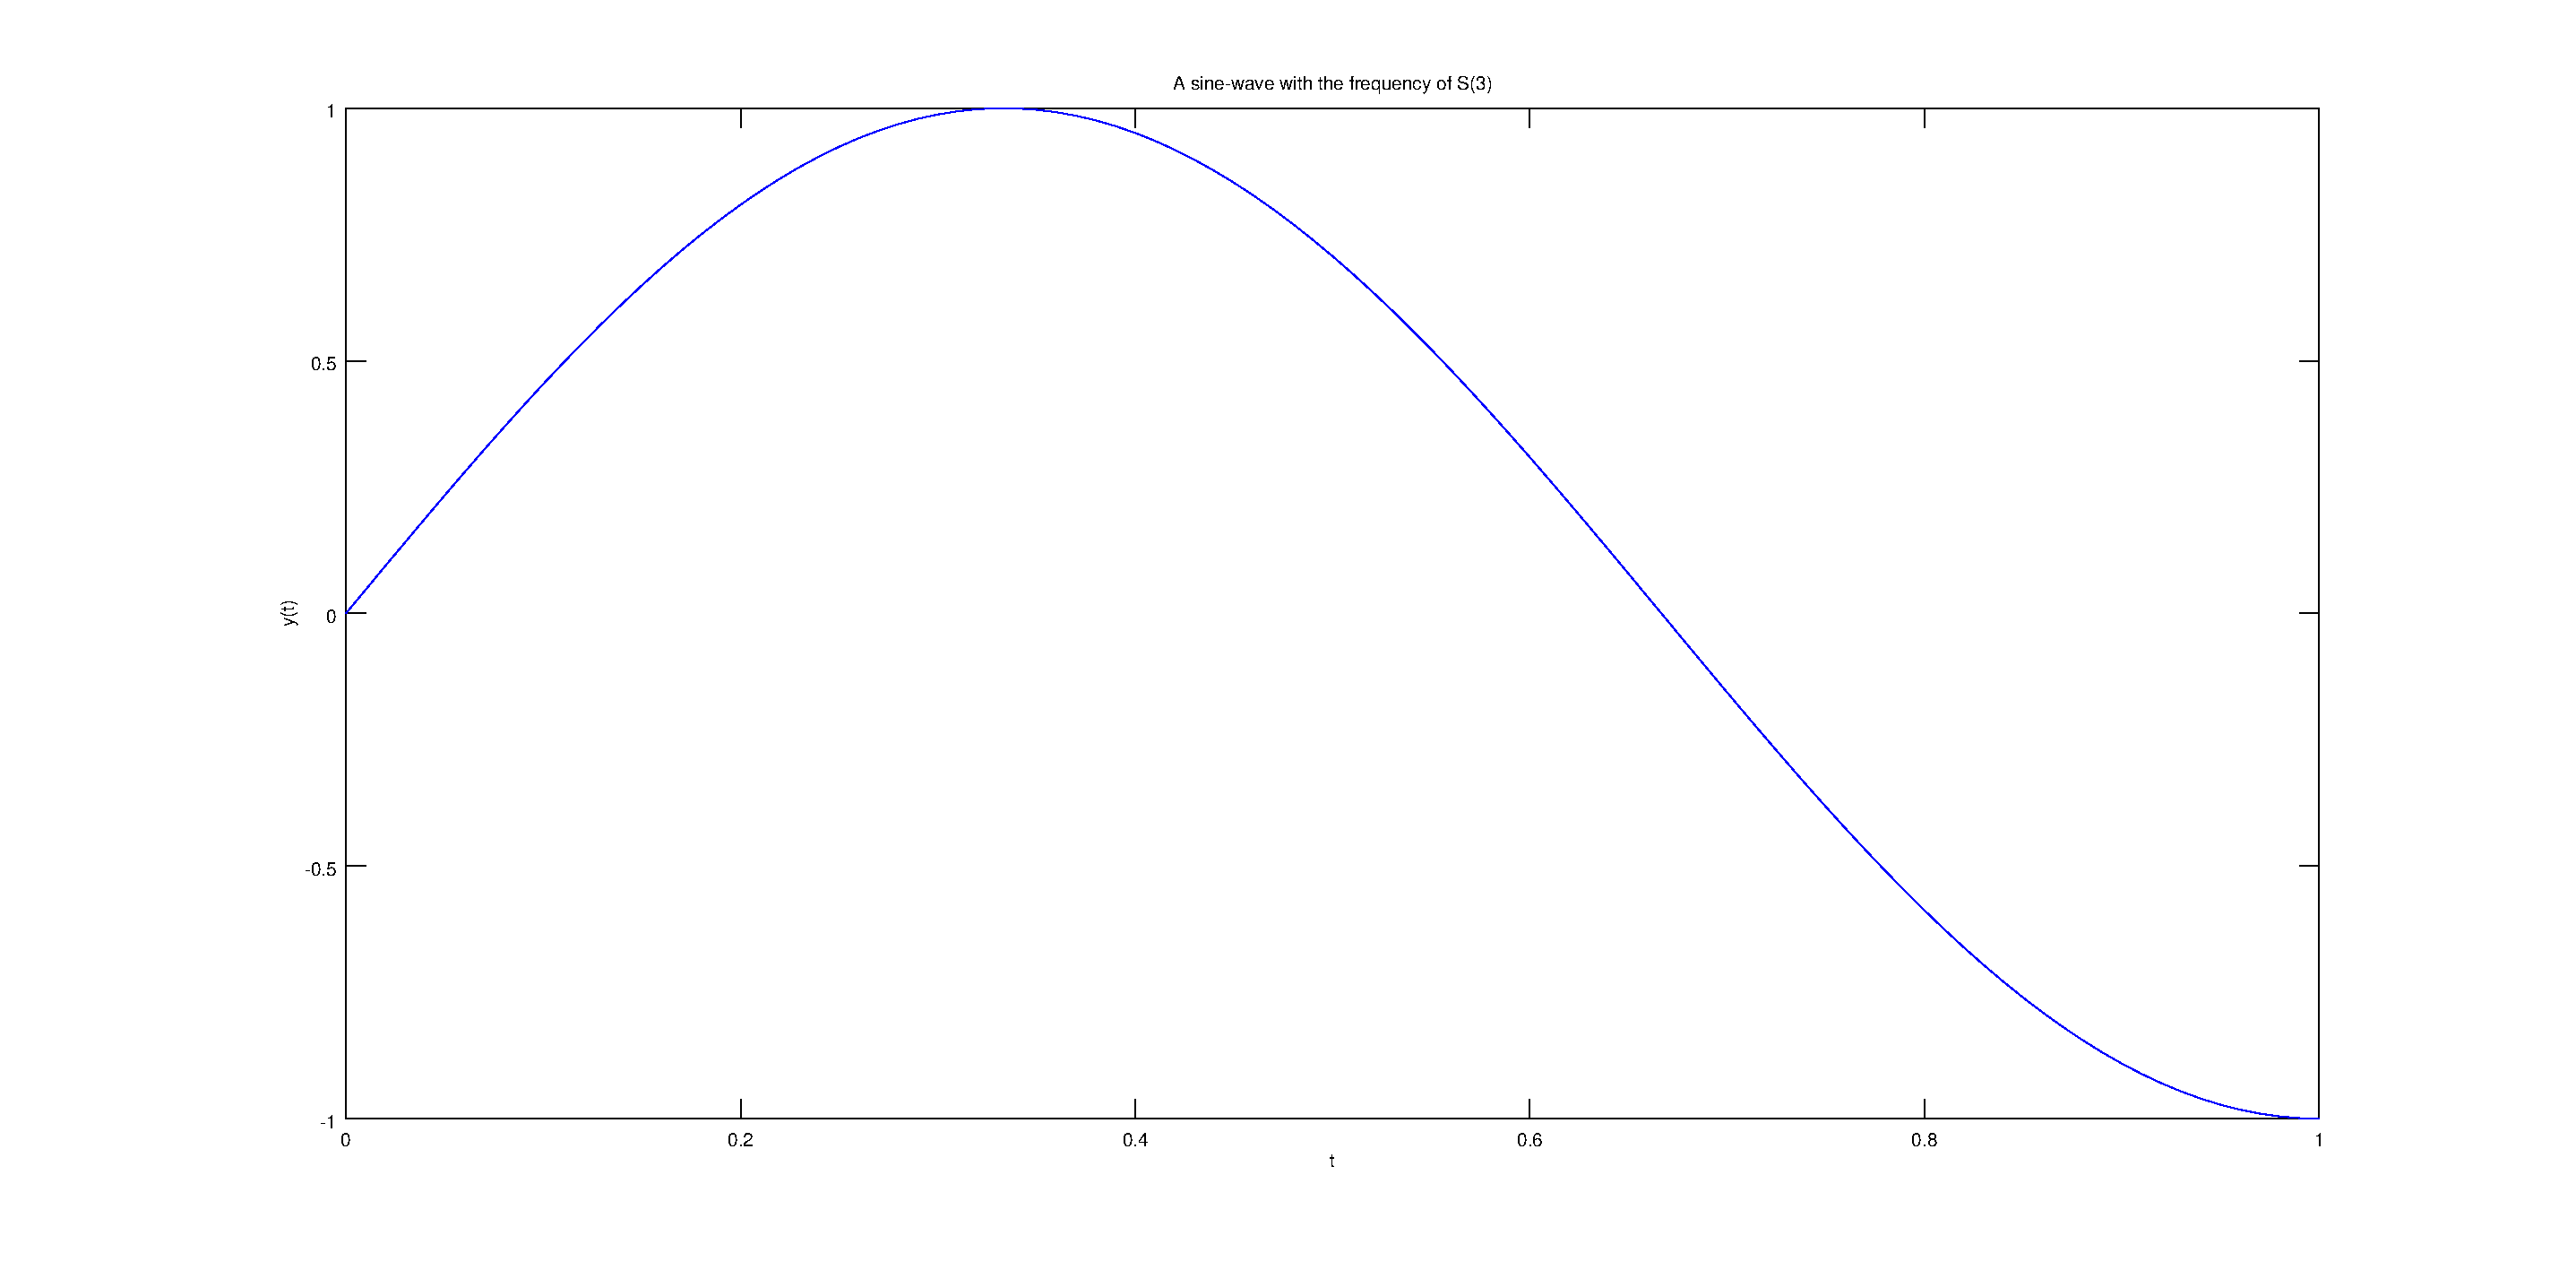
\includegraphics[clip,width=\textwidth]{frequency.eps}
        \caption{Output of the second part of the Matlab script}
    \end{figure}
    \subsection{}
    \lstinputlisting[firstline=27,firstnumber=27,lastline=35]{sh02ex02.m}              
    \subsection{}
    \lstinputlisting[firstline=36,firstnumber=36]{sh02ex02.m}              
    \begin{figure}[H]
        \centering
        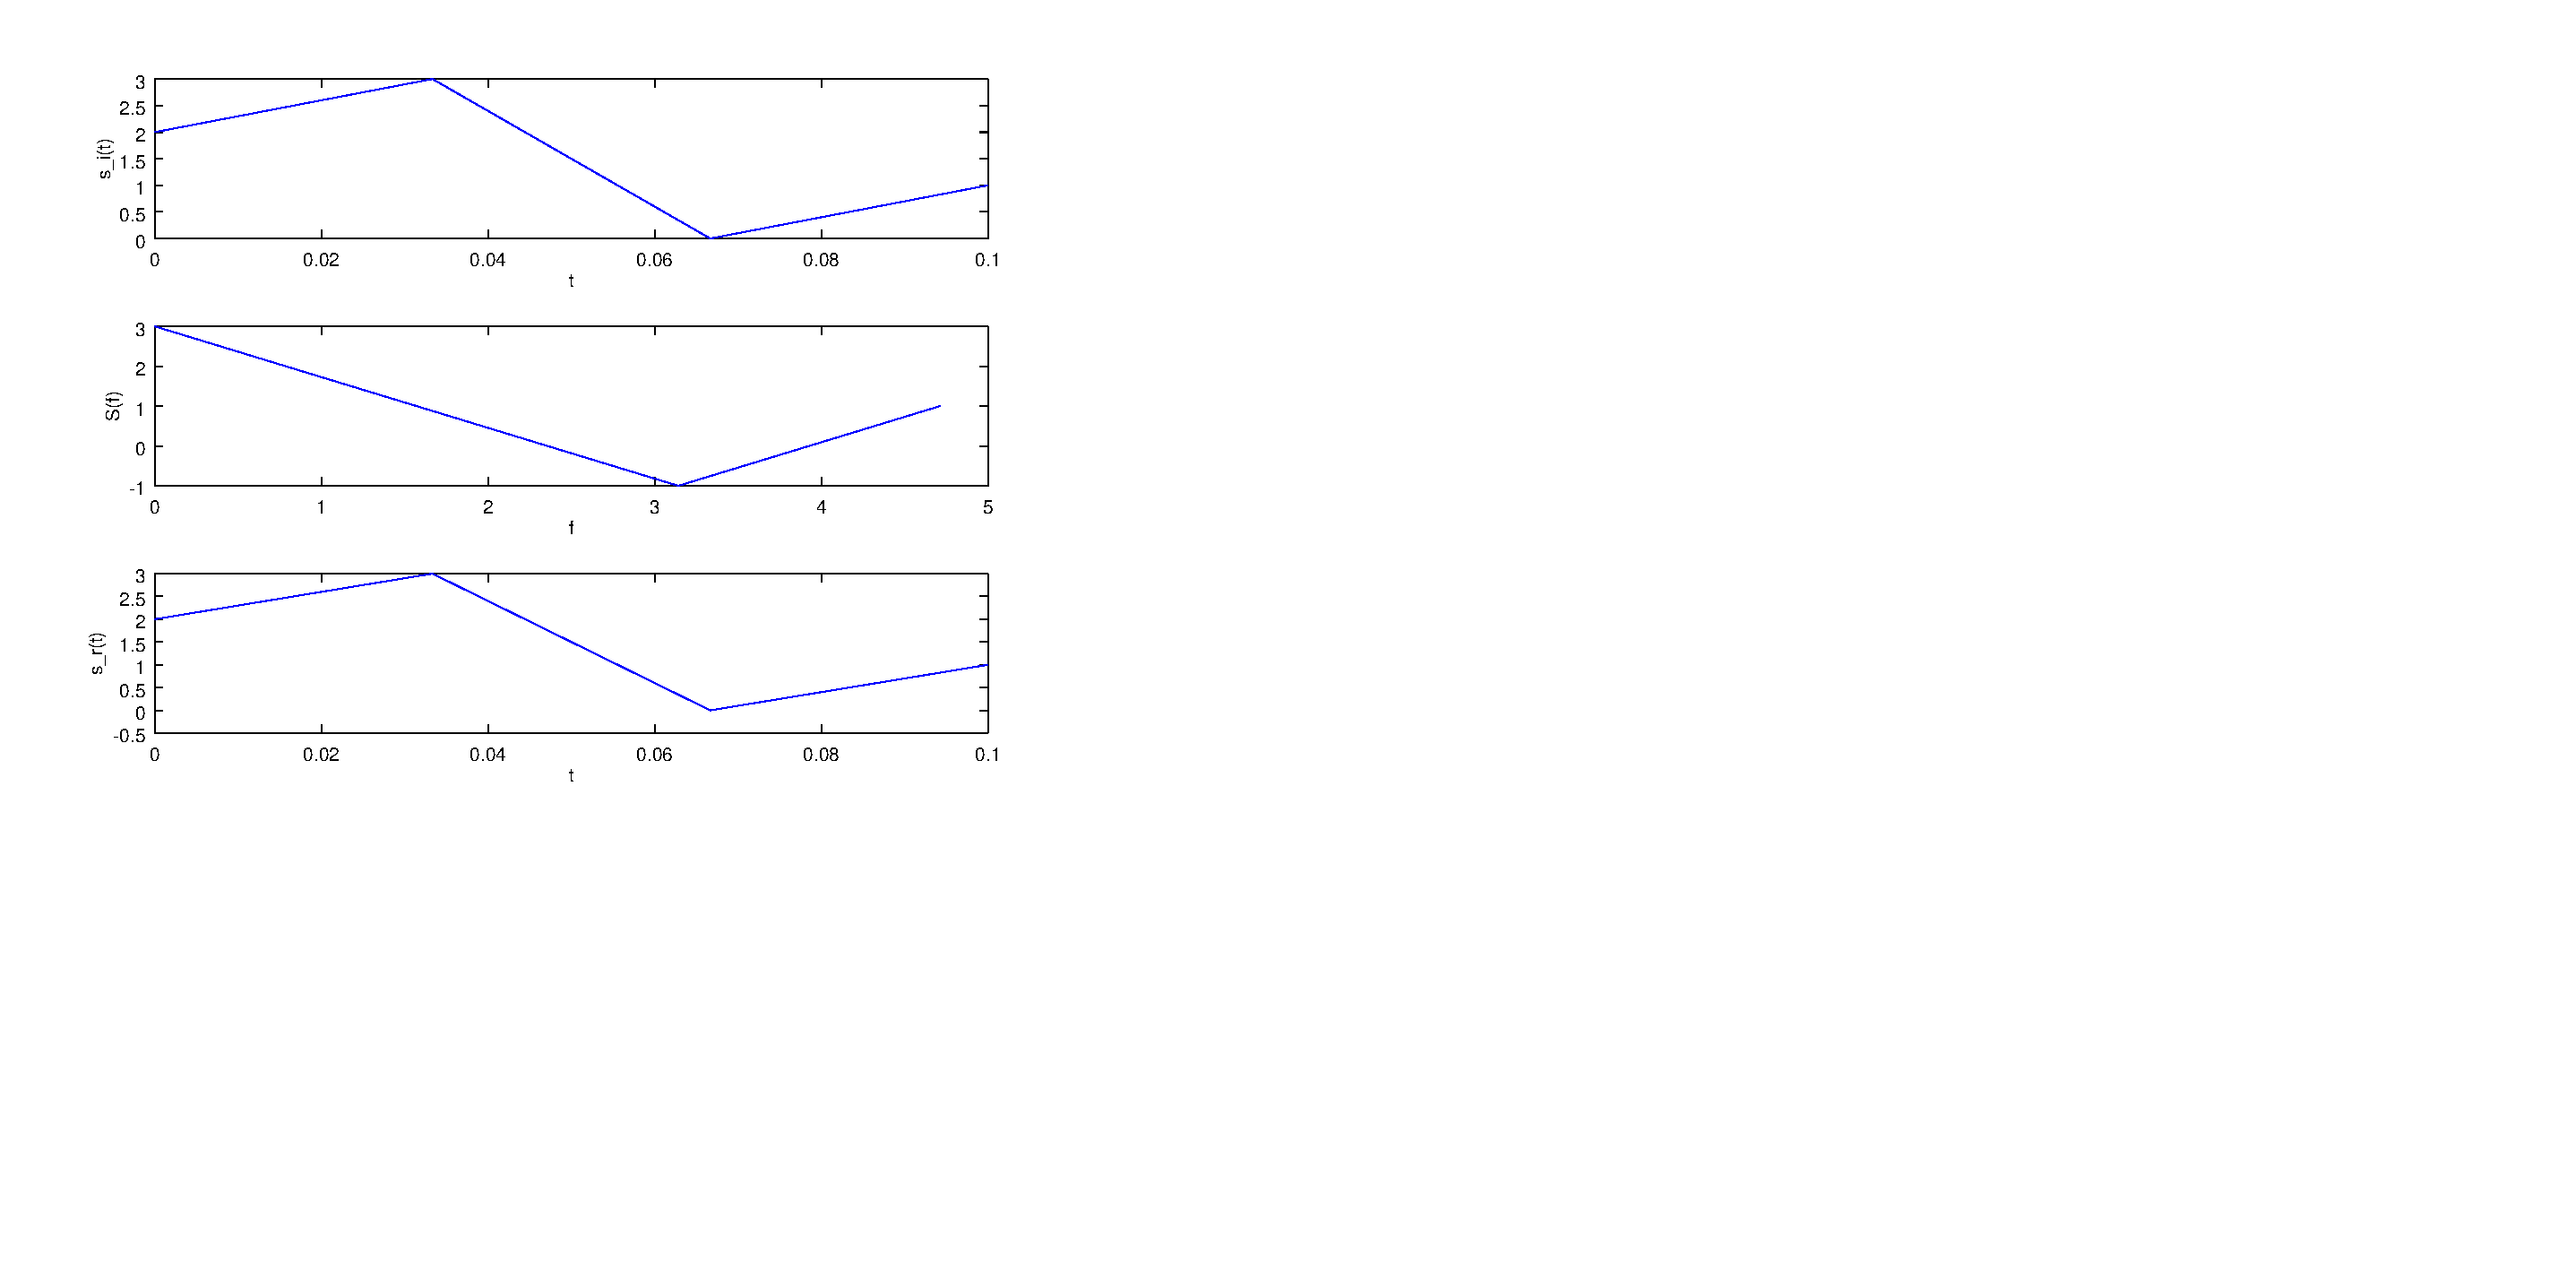
\includegraphics[trim = {0 8cm 27cm 0}, clip,width=\textwidth]{transforms.eps}
        \caption{Output of the last part of the Matlab script}
    \end{figure}

    \section{Fourier Transform for Image Quality Assessment}
    \subsection{}
    \lstinputlisting[lastline=10]{sh02ex03.m}              
    \subsection{}
    \lstinputlisting[firstline=11,firstnumber=11,lastline=20]{sh02ex03.m}              
    \subsection{}
    \lstinputlisting[firstline=21,firstnumber=21,lastline=27]{sh02ex03.m}              
    \subsection{}
    \lstinputlisting[firstline=28,firstnumber=28]{sh02ex03.m}              
    \begin{figure}[H]
        \centering
        \includegraphics[trim = {0 8cm 27cm 0}, clip,width=\textwidth]{Quality.eps}
        \caption{Output of the Matlab script}
    \end{figure}
\end{document}
